% !TeX encoding = UTF-8
% !TeX spellcheck = pl_PL
\chapter{Wskazówki i przykłady}

W rozdziale tym zamieszczono szereg wskazówek i przykładów formatowania  w~{\LaTeX}-u typowych elementów pracy dyplomowej. Tekst źródłowy przykładów można skopiować i~przystosować do własnych potrzeb.

\section{Formatowanie tekstu}
\subsection{Font, style, itd.}
Font, stopień pisma tekstu i tytułów rozdziałów, wielkość wcięć i odstępów, itd. ustala sam {\LaTeX} na podstawie definicji zawartych w szablonie dokumentu. Użytkownik nie musi niczego definiować samodzielnie.

\subsection{Akapity}
Akapit nie wymaga  specjalnego formatowania. Tekst należy wpisywać bez wymuszania przejścia do nowego wiersza czyli tzw. ręcznego wstawiania znaków powrotu karetki. Liczba                       odstępów                        pomiędzy wyrazami,              tzw. \textit{spacji},   większa niż jeden jest  interpretowana jak jeden odstęp.

W celu rozpoczęcia  nowego akapitu należy pozostawić wiersz odstępu. Wszystkie parametry tekstu takie jak wcięcia akapitowe, odstępy między wierszami i~między akapitami  ustawia sam  {\LaTeX}. 

Należy pamiętać, aby nie pozostawiać na końcu wiersza samotnego spójnika (np.:~"i", "a", "z").  W tym celu pomiędzy spójnik i następny wyraz należy wstawić tzw. "niełamliwy" odstęp. W  \mbox{{\LaTeX}-u} uzyskuje się taki odstęp przez umieszczenie pomiędzy wyrazami znaku "\textasciitilde" zamiast zwykłego odstępu, np. "w\textasciitilde tekście".


\subsection{Wstawianie specjalnych symboli}
Obecnie, dzięki pakietom językowym, nie ma potrzeby stosowania tzw. \textit{escape codes}  w celu uzyskania znaków narodowych (np.  \texttt{\textbackslash k\{a\}} dla uzyskania ą). Wystarczy zapisać tekst w pliku z kodowaniem UTF-8 oraz użyć odpowiedniego pakietu, np:
{\footnotesize \begin{verbatim}
\usepackage{polyglossia}
\setdefaultlanguage[]{polish}
\end{verbatim}
}

Często zachodzi potrzeba wstawienia symbolu, np. litery z greckiego alfabetu. Rozwiązanie tego problemu zależy od tego w jakim elemencie tekstu chcemy uzyskać taki symbol. 

Jeśli symbol występuje we wzorze to rozwiązaniem jest zastosowanie trybu matematycznego  (szczegóły w rozdziale \ref{sec:wzory}), w którym pożądany symbol wstawiamy za pomocą specjalnego kodu, np.: \texttt{\textbackslash mu} -- $\mu $, \texttt{\textbackslash pi}~--~$\pi$.

Jeśli symbol jest nazwą jednostki to wtedy można "awaryjnie" zastosować tryb matematyczny. Powstaje formuła osadzona w tekście, np. 3~$\mu m$. Jednak znacznie lepiej jest zastosować specjalne polecenia z pakietu \texttt{siunitx} uzyskując napis \SI{3}{\micro\meter}. Szczegóły w rozdziale \ref{sec:liczby}.

\subsection{Wyróżnianie tekstu}
W celu wyróżnienia fragmentu tekstu można zastosować \textit{specjalną odmianę  kroju czcionki zwaną italikiem}, \textbf{wytłuszczenie}  lub  \underline{podkreślenie}. Należy pamiętać, żeby nie nadużywać tej formy ekspresji. Zaleca się wybranie jednej z~tych metod wyróżniania tekstu i  konsekwentne jej stosowanie w całej pracy. Wytłuszczenia są często zarezerwowane dla oznaczania wektorów, macierzy, itd. Dlatego zwykłe wyróżnienie tekstu najlepiej zrealizować   \textit{przez zastosowanie italików}. 




\subsection{Wyliczenia}
Wyliczenia, zwane też listami, tworzymy korzystając  z otoczeń (ang.~\textit{environments}). {\LaTeX}  formatuje listy całkowicie automatycznie.  Najczęściej stosuje się dwa rodzaje list:
\begin{itemize}
\item \textit{nieuporządkowaną}, uzyskiwaną przez użycie otoczenia \texttt{itemize},
\item \textit{uporządkowaną}, uzyskiwaną przez użycie otoczenia \texttt{enumerate}.
\end{itemize}
Podczas składania list należy pamiętać o stosowaniu poprawnej interpunkcji. Poniżej dwa przykłady wyliczeń:
\begin{itemize}
\item Nieuporządkowana poziom pierwszy, 
\begin{itemize}
\item nieuporządkowana poziom drugi,
\begin{itemize}
\item nieuporządkowana poziom trzeci.
\end{itemize}
\end{itemize}
\end{itemize}

\begin{enumerate}
\item  Uporządkowana poziom pierwszy,
\begin{enumerate}
\item uporządkowana poziom drugi,
\begin{enumerate}
\item uporządkowana poziom trzeci.
\end{enumerate}
\end{enumerate}
\end{enumerate}




\subsection{Liczby}
\label{sec:liczby}
Liczby i miana należy sformatować zgodnie z zasadami typografii obowiązującymi w języku polskim oraz zgodnie z normami SI. Częstym błędem jest podawania wartości liczbowych w taki sposób w jaki wyświetlają je symulatory, np. 3.3V zamiast 3,3~V.  Należy zwrócić uwagę na stosowanie właściwego znaku oddzielającego część całkowitą od ułamkowej oraz na oddzielanie miana od samej liczby (najprostszym sposobem jest wstawienie pomiędzy liczbę i symbol tzw. niełamliwej spacji czyli tyldy). 

Problem formatowania liczb można rozwiązać w bardziej ogólny sposób używając pakietu \texttt{siunitx}.  Pakiet ten zawiera szereg poleceń, od prostych służących do formatowania liczb: \num{123e-5}, \ang{100}, \SI{1050}{\degreeCelsius}, \SI{1}{\micro\meter} aż po bardziej złożone służące do justowania liczb w tabelach.
\begin{table}[!h]
\caption{Przykład wykorzystania pakietu \texttt{siunitx} do justowania zawartości pól tabeli.}
\centering
  \begin{tabular}{@{}lS[table-format=3.2]>{\bfseries}S[table-format=3.2]@{}}
    \toprule
    \textbf{Foo} & \textbf{Normal} & \textbf{Bold} \\
    \midrule
    foo1 & 111 & 111 \\
    foo2 & 222.2 & 222.2 \\
    foo3 & 3.33 & 3.33 \\
    foo4 & 4 & 4 \\
    foo5 & 5.5 & 5.5 \\
    \bottomrule
  \end{tabular}
\end{table}


\subsection{Adresy internetowe}
Adresy internetowe formatujemy za pomocą polecenia \textbackslash url\{\textit{adres}\}, np. \url{http://www.tug.org/}.

\section{Przypisy}
Jeśli trzeba utworzyć przypis to w {\LaTeX}-u\footnote{{\LaTeX} - (od [Leslie] Lamport {\TeX}) oprogramowanie do zautomatyzowanego składu tekstu.}  korzystamy z instrukcji \texttt{ \textbackslash footnote\{\textit{przypis}\}}.

\section{Odsyłacze}
W tekście pracy dyplomowej często umieszcza się odniesienia do ilustracji, tabel, wzorów lub podrozdziałów.  {\LaTeX} sam zajmuje się generacją numeracji tych elementów. Tak więc na etapie tworzenia tekstu konkretne indeksy nie są jeszcze znane. Dlatego w tekście wstawia się odsyłacze do etykiet a same etykiety umieszcza w definicjach elementów, do których zamierzamy się odnosić.

Etykietę tworzy się za pomocą polecenia \texttt{\textbackslash label\{\textit{etykieta}\}}. Warto przemyśleć system tworzenia nazw etykiet tak, aby łatwo kojarzyły się z typem obiektu. Przykładowo, etykieta ilustracji zawiera prefiks \textit{fig:} (np. \textbackslash label\{fig:fdota\}) a ~etykieta wzoru  prefiks \textit{Eq:} (np. \textbackslash label\{Eq:ulamek\}). 

Odsyłacz powstaje poprzez umieszczenie polecenia \texttt{\textbackslash ref\{\textit{etykieta}\}} (np.~\textbackslash ref\{fig:fdota\}). A~oto przykłady zastosowania odsyłacza do rysunku: Rys.~\ref{fig:fdota}, wzoru  \ref{Eq:frac} i rozdziału \ref{sec:wzory}.

\section{Tabele}
Tabele składamy korzystając z otoczenia \texttt{tabular}. Podstawowe zasady składania tabel są proste i ich zastosowanie w praktyce nie powinno sprawiać trudności.  Jednak w przypadkach bardziej złożonych struktur (np. łączenie pól, kolumn, wierszy) czy też tabel wykraczających poza jedną stronę może się okazać, że konieczne będzie zastosowanie specjalnych pakietów {\LaTeX}-a. Przedstawienie zaawansowanych metod składania tabel wykracza poza zakres tego dokumentu. Zainteresowanych odsyłam do dokumentacji. Zawsze warto skorzystać ze wsparcia jakiego w tym zakresie udzielają wyspecjalizowane narzędzia na przykład wspominany już w~rozdziale~\ref{sec:tools} program \mbox{\textit{TeXstudio}}.     
\begin{table}[!h]
\caption{Przykładowa tabela -- zawartość pól wyśrodkowana.}
\centering
\begin{tabular}{|c||c|c|c|c|}
\hline & Nagłówek 1  & Nagłówek 2  & Nagłówek 3  &  Nagłówek 4 \\ 
\hline
\hline  Etykieta wiersza & bb bb bbbb bbbb  & cc  & dd   &  ee  \\
\hline  Etykieta wiersza & bb  & cc  & dd   &  ee \\
\hline  Etykieta wiersza  & bb  & cc  & dd   &  ee \\ 
\hline  Etykieta wiersza  & bb  & cc  & dd   &  ee ee eeee  eeeee\\
\hline 
\end{tabular} 
\label{tab:tab2}
\end{table}

\begin{table}[!h]
\caption{Przykładowa tabela -- wyrównywanie zawartości pól do lewego lub prawego  marginesu.}
\centering
\begin{tabular}{|l|l|r|}
\hline  Nagłówek 1  &  Nagłówek 2  &  Nagłówek 3  \\ 
\hline
\hline  bb bb bbbb bbbb   & dd   &  ee  \\
\hline   cc  & dd   &  ee ee eeee  eeeee\\
\hline 
\end{tabular} 
\label{tab:tab3}
\end{table}

\begin{table}[!h]
\centering
\caption{Przykład tabeli z diagonalnym podziałem komórki.}
\label{tab:time}
\begin{tabular}{|c|c|c|}
\hline
\diagbox{Etykieta wierszy}{Etykieta kolumn}  &  Nagłówek 1  & Nagłówek 2\\
\hline Nagłówek 1  &  Nagłówek 2  &  Nagłówek 3 \\ 
\hline AAAAA AAAAA & BBBB BBB & CCCC CCCC \\
\hline AAAAAA & 2 & 3 \\
\hline
\end{tabular}
\label{tab:tabdiag}
\end{table}

\begin{table}[!h]
\caption{Wymuszenie konkretnych  szerokości kolumn.}
\centering
\begin{tabular}{|l|l|p{25mm}|l|p{3cm}|}
\hline & Nagłówek 1  & Nagłówek 2  & Nagłówek 3  &  Nagłówek 4  \\ 
\hline
\hline  Etykieta wiersza & bb  & cc  & dd   &  Podstawowe zasady składania tabel są proste i ich zastosowanie w praktyce nie powinno sprawiać trudności \\
\hline  Etykieta wiersza  & bb  & cc cc cccc cccccc  & dd   &  ee \\ 
\hline 
\end{tabular} 
\label{tab:tab1}
\end{table}


\newpage
\section{Cytowanie kodu źródłowego}
Cytując kod programu czy też modelu HDL najlepiej jest skorzystać z pakietu \texttt{listings}, który definiuje otoczenie  \texttt{\textbackslash begin\{lstlisting\}}\dots\texttt{ \textbackslash end\{lstlisting\}}. Pakiet ten pozwala na automatyczne wyróżnianie słów kluczowych szeregu języków  programowania i opisu sprzętu. Poniżej pokazano przykłady: modelu VHDL (wydruk~\ref{lst:latch}), modelu Verilog (wydruk~\ref{lst:adder}) oraz programu w języku C++(wydruk~\ref{lst:hello}).

  
\begin{lstlisting}[language=VHDL, caption={Przykładowy model VHDL}, label={lst:latch}]
entity latch is
port (sample: in std_logic;
count : in  std_logic_vector (0 to 7);
data:   out std_logic_vector (0 to 7));
end latch;

architecture behav of latch is     -- zatrzask
begin
process (sample, count)
begin
	if (sample = '1') then
		data <= count;
	end if;
end process;
end behav;
\end{lstlisting}



\begin{lstlisting}[language=Verilog, caption={Przykładowy model Verilog}, label={lst:adder}]
module add_carry_signed_final (
input signed [2:0] A,
input signed [2:0] B,
input carry_in,
output signed [3:0] Sum);

assign Sum = A + B + $signed({1'b0, carry_in});

endmodule
\end{lstlisting}


\begin{lstlisting}[language=c++, caption={Przykładowy program C++}, label={lst:hello}]
// 'Hello World!' program 

#include <iostream>

int main()
{
	std::cout << "Hello World!" << std::endl;
	return 0;
}
\end{lstlisting}



\section{Ilustracje}
\label{sec:ilustracje}
Ilustracje są pobierane z plików, przy  czym preferowany jest format PDF lub PNG.
\subsection{Przygotowanie ilustracji}
O ile to możliwe ilustracje powinny być przygotowane w~postaci wektorowej, przy pomocy niezależnego oprogramowania i zapisane w plikach o formacie PDF lub SVG (ten drugi wariant wymaga lepszej znajomości {\LaTeX}-a). Zaawansowani użytkownicy mogą wykorzystać pakiety TikZ i PGF (\url{http://sourceforge.net/projects/pgf/}). 

Jeśli ilustracja dostępna jest tylko w wersji rastrowej (np. plik graficzny zawierający przebiegi uzyskane w trakcie  symulacji) to należy użyć formatu pliku o~bezstratnej kompresji a~zastosowana rozdzielczość  nie może być mniejsza niż 300~dpi a najlepiej 600~dpi. 

\textit{Uwaga! Tzw. zrzuty ekranowe mają rozdzielczość taką jak obraz na ekranie monitora czyli zwykle mniej niż 100~dpi i nie prezentują się dobrze na wydrukach.}   

Przygotowując ilustracje trzeba pamiętać, że zastosowany w nich font i stopień pisma musi być zgodny z wyglądem tekstu. Stosujemy ten sam font co w tekście (lub jeśli to niemożliwe, inny o podobnym kroju) a~wielkość napisów powinna być nieco mniejsza niż w tekście (jeśli stopień pisma tekstu wynosi 11~pt to ilustracje mogą stosować np. 9~pt). Można też zastosować w ilustracjach  font  bezszeryfowy (takich jak np.~Arial). Niezależnie od tego jaką konwencję przyjmiemy należy \textit{stosować ją konsekwentnie do wszystkich ilustracji}.

Kolejna kwestia to fizyczny rozmiar ilustracji. Przygotowywana grafika powinna mieć takie fizyczne wymiary, aby w~trakcie włączania jej do dokumentu nie dokonywać skalowania. Skalowanie bardzo źle wpływa na czytelność grafiki rastrowej. Ponadto skalowanie zmienia grubość linii i wielkość napisów. Jeśli nie zastosuje się jednakowych zasad to może się okazać, że ilustracje nie prezentują się w jednolity sposób co sprawia fatalne wrażenie.

\subsection{Składanie ilustracji}
Ilustracje mogą być zamieszczane pojedynczo (Rys.~\ref{fig:fdota}) lub, jak pokazano na Rys.~\ref{fig:otah1},  obok siebie korzystając z otoczenia \texttt{tabular} (Rys.~\ref{fig:otah1}). Można też  zastosować polecenie \textbackslash \texttt{subfloat}.
\begin{figure}[!h]
\begin{center}
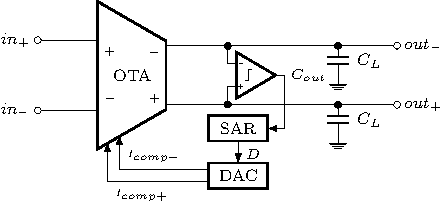
\includegraphics[scale=1]{fdota.pdf}\\
\end{center}
\caption 
{ \label{fig:fdota} 
Schemat blokowy FDOTA z cyfrową kalibracją napięcia niezrównoważenia.}
\end{figure}
\begin{figure}[!h]
  \begin{center}
  	\setlength{\tabcolsep}{0pt}
  	\begin{tabular}{ll}
  		(a) & (b)\\
  		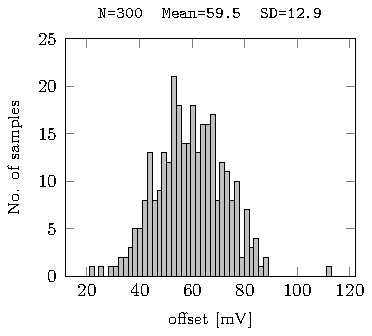
\includegraphics[height=5.2cm]{hist1.pdf}&
  		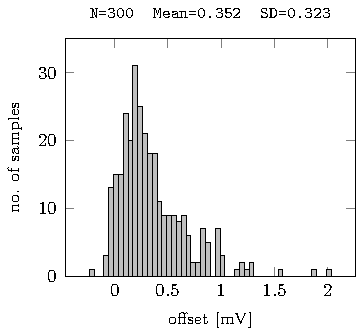
\includegraphics[height=5.2cm]{hist2.pdf}\\
  	\end{tabular}
  \end{center}
\caption
{ \label{fig:otah1} 
Rozrzut napięcia niezrównoważenia FDOTA: (a) bez kalibracji, (b) z 9-bitową kalibracją.}
\end{figure} 


\pagebreak


\section{Składanie wzorów}
\label{sec:wzory}
Jedną z wielu zalet {\LaTeX}-a, jak przystało na system składu publikacji naukowych, jest tryb matematyczny. W tym podrozdziale pokazano szereg przykładów użycia podstawowych konstrukcji tego trybu.

\subsection{Formuły w osobnych wierszach}
Podstawowym sposobem składania wzorów jest umieszczanie ich w osobnym wierszu. Wzory powinny być numerowane, tak jak to widać w poniższy przykładzie:
\begin{equation}
y= \frac{x-1}{x+2} 
\end{equation}
Automatyczną numerację uzyskujemy stosując otoczenie \texttt{\textbackslash begin\{equation\}\dots\textbackslash end\{equation\}}.
Umieszczenie etykiety umożliwi łatwe odwoływanie się do wzoru w~tekście, np. do formuły \ref{Eq:frac}.

\subsection{Formuły osadzone w tekście}
W najprostszym przypadku wzory mogą być integralną częścią akapitu, np. $E=mc^2$. Trzeba jednak pamiętać, że takie rozwiązanie stosujemy tylko do bardzo prostych (pomocniczych) zależności. Taka formuła jest trudna do odnalezienia, nie można uzyskać do niej odsyłacza a jeśli jest bardziej rozbudowana "rozpycha" tekst.

Szczególnie niekorzystnie  prezentują się osadzone w tekście ułamki ze względu na zmniejszony stopień pisma,  np. $y= \frac{x-1}{x+2}$. Jeśli zdecydujemy się temu zaradzić stosując polecenie \texttt{dfrac} zamiast \texttt{frac}, np.:  $y=\dfrac{x-1}{x+2}$, to znacząco zaburzona zostanie wielkość odstępów międzywierszowych, przez co tekst prezentuje się w sposób mało profesjonalny.

\subsection{Ułamki z ukośnikiem}
Proste ułamki lub miana można zapisać z wykorzystaniem ukośnika, np.: $\sfrac{1}{3}$, $\sfrac{1}{n}$, $\sfrac{V}{A}$.



\subsection{Indeksy górne i dolne}
Często spotykane są wyrażenia, w których stosowane są indeksy górne i dolne, np.:
\begin{equation}
a_{1},\ a_{i_{1}},\ a^{2},\ a^{b^{c}},\ a^{i_{1}},\
a_{i} + 1,\ a_{i + 1},\ a_{2}^{1},\ a^{2}_{1}
\end{equation}


\begin{equation}
x_{1} + x_{2} + \dots + x_{n}
\end{equation}


\subsection{Nawiasy i ograniczniki}
Szereg symboli takich jak nawiasy występuje w kilku odmianach różniących się wielkością. np.:
\[
( \dots \big( \dots \Big( \dots \bigg( \dots \Bigg(
\]
Zastosowanie "dużych" symboli poprawia czytelność złożonych formuł, np.: 
\[
F(x) |^{b}_{a} \dots
F(x) \bigr|^{b}_{a} \dots
F(x) \Bigr|^{b}_{a}
\]

\[
[ \sum_i a_i ]^{1/p} \dots  \left[ \sum_i a_i \right]^{1/p} \dots  \bigg[ \sum_i a_i \bigg]^{1/p} \dots  \Bigg[ \sum_i a_i \Bigg]^{1/p}
\]


\section{Ułamki piętrowe}

Zastosowanie zwykłego polecenia \texttt{frac} nie daje dobrych rezultatów:
\begin{equation}
  x = a_0 + \frac{1}{a_1
          + \frac{1}{a_2
          + \frac{1}{a_3 + \frac{1}{a_4} } } }
\end{equation}
W takiej sytuacji należy zastosować instrukcję \texttt{cfrac}:
\begin{equation}
  x = a_0 + \cfrac{1}{a_1
          + \cfrac{1}{a_2
          + \cfrac{1}{a_3 + \cfrac{1}{a_4} } } }
\end{equation}

\section{Justowanie wzorów}
Jeśli w tekście występuje kolejno kilka formuł to powinny one być wyjustowane względem siebie. Efekt ten uzyskuje się za pomocą otoczenia \texttt{\textbackslash begin\{align\}\dots\textbackslash end\{align\}}. W~formułach umieszczany jest symbol "\&", którego położenie wyznacza punkt odniesienia w każdej z~nich. Poniżej kilka przykładów wyjustowanych formuł.
\begin{align}
r^{2} &= s^{2} + t^{2}, \label{Eq:Pyth}\\
2u + 1 &= v + w^{\alpha}, \label{Eq:alpha}\\
x &= \frac{y + z}{\sqrt{s + 2u}};\label{Eq:frac}
\end{align}
\begin{align}
h(x) &= \int \left( \frac{f(x) + g(x)}{1+ f^{2}(x)} + \frac{1+ f(x)g(x)}{\sqrt{1 - \sin x}} \right) \, dx\label{E:longInt}=\\
&= \int \frac{1 + f(x)}{1 + g(x) } \, dx - 2 \tan^{-1}(x-2)\notag
\end{align}
W niektórych przypadkach samo justowanie nie wystarcza, np. podczas składania wzoru funkcji określonej przedziałami. W takim przypadku korzystamy z otoczenia \texttt{\textbackslash begin\{cases\}\dots \textbackslash end\{cases\}}. 
\begin{equation}
f(x)=
\begin{cases}
-x^{2}, &\text{if $x < 0$;}\\
\alpha + x, &\text{if $0 \leq x \leq 1$;}\\
x^{2}, &\text{otherwise.}
\end{cases}
\end{equation}



\section{Ingerowanie w skład dokumentu}
{\LaTeX} stara się rozmieścić tekst i inne elementy takie jak tabele, ilustracje czy wzory tak, aby uzyskać najlepszy efekt. Zdarza się jednak, np. kiedy blisko siebie występuje  duża liczba rysunków, że trzeba zaingerować  w układ pracy. 
\subsection{Kotwiczenie rysunków i tabel}
Jedną z najczęściej spotkanych sytuacji jest wymuszenie konkretnej pozycji ilustracji lub tabeli. W~tym celu należy definicję obiektu, czyli otoczenie \texttt{table} lub \texttt{figure}, uzupełnić o opcje wskazujące pożądaną lokalizację obiektu: \texttt{\textbackslash begin\{table\}\textbf{[!h]}},	\texttt{\textbackslash begin\{figure\}\textbf{[!h]}}. Litera \textit{h} jest skrótem od \textit{here}. Wykrzyknik nakazuje zaniechanie stosowania standardowych reguł rozmieszczania rysunków i tabel.

\subsection{Wymuszanie złamania strony}
Można wymusić złamanie strony w~konkretnym miejscu wstawiając polecenie  \texttt{\textbackslash pagebreak[\textit{n}]} (gdzie opcjonalny parametr \textit{n}=1\dots 4), które  {\LaTeX} interpretuje jako życzenie by zakończyć w tym miejscu stronę, tym silniejsze im większa jest wartość \textit{n}. 

\subsection{Wymuszanie złamania wiersza}
W celu wymuszenia przejścia do nowego wiersza \textit{bez rozpoczynania nowego akapitu} można zastosować polecenie \texttt{\textbackslash\textbackslash} lub \texttt{\textbackslash newline}.

\subsection{Zapobieganie wstawianiu wcięcia akapitowego}
Czasem (np. w sytuacji cytowania w podrozdziale \ref{fonty}) chcemy wstawić wiersz odstępu i jednocześnie uniknąć rozpoczęcia nowego akapitu. Wtedy na początku bloku tekstu wstawiamy polecenie \texttt{\textbackslash noindent}.

\subsection{Zapobieganiu przenoszeniu do nowego wiersza}
{\LaTeX} składając akapity stosuje automatyczne dzielenie i przenoszenie wyrazów, zgodnie z~regułami obowiązującymi w~języku, w jakim tworzony jest dokument. Zdarza się niekiedy, że zostaje rozdzielony   w ten sposób tekst, którego nie chcemy dzielić, np.: adres internetowy, stała fizyczna, itp. Można zapobiec dzieleniu słów i~przenoszeniu do nowego wiersza umieszczając tekst jako argument polecenia  \texttt{\textbackslash mbox\{\dots \}}. Poniżej przykład takiej sytuacji.
\vskip12pt
\textit{TeXstudio} jest dostępne nieodpłatnie na wszystkie platformy systemowe  na \url{http://texstudio.sourceforge.net/}.
\vskip12pt
\textit{TeXstudio} jest dostępne nieodpłatnie na wszystkie platformy systemowe  na \mbox{\url{http://texstudio.sourceforge.net/}}.

\subsection{Znaki specjalne}
Zdarza się że, musimy użyć słowa, które zawiera znak specjalny {\LaTeX}-a. Przykładem takiej sytuacji jest cytowanie nazwy pliku, która zawiera znak podkreślenia  "\_", np. w nazwie pliku \textit{praca\_dyplomowa.tex}. Wtedy należy taki znak poprzedzić odwróconym ukośnikiem czy znakiem \textbackslash.

\newpage
\section{Spis literatury}
Spis literatury generowany jest automatycznie, na podstawie umieszczonych w tekście odsyłaczy do rekordów bazy bibliograficznej.  
\subsection{Baza bibliograficzna w formacie \BibTeX}
Baza bibliograficzna w formacie \BibTeX jest w istocie plikiem tekstowym (o nazwie zwyczajowo zakończonej przez rozszerzenie \texttt{.bib}) zawierającym rekordy opisujące poszczególne pozycje. Praktycznie wszystkie wydawnictwa dostarczają referencji w formacie  \BibTeX, tak więc skompletowanie odpowiednio sformatowanej bazy bibliograficznej nie będzie nastręczało żadnych trudności. Każdy rekord w bazie musi zawierać  identyfikujący go unikalny klucz (etykietę). W podanym poniżej przykładzie są to \texttt{Pastre2006}, \texttt{Pastre2009}, \texttt{Pelgrom1989} i \texttt{wikibook}. 

{\footnotesize \begin{verbatim} 
@BOOK{Pastre2006,
  author = {Marc Pastre and Maher Kayal},
  title = {Methodology for the Digital Calibration of Analog Circuits and Systems: with 
  Case Studies (The Springer International Series in Engineering and Computer Science)},
  year = {2006},
  publisher = {Springer},
  isbn = {1402042523},
  url = {http://www.amazon.com/Methodology-Digital-Calibration-Circuits-Systems/dp/}
}
@INPROCEEDINGS{Pastre2009,
  author = {Pastre, M. and Kayal, M.},
  title = {Methodology for the digital calibration of analog circuits and systems 
  using sub-binary radix DACs},
  booktitle = {Mixed Design of Integrated Circuits Systems, 2009. MIXDES '09. MIXDES-16th
  International Conference},
  year = {2009},
  pages = {456-461},
  keywords = {analogue integrated circuits;calibrationy}
}
@ARTICLE{Pelgrom1989,
  author = {Pelgrom, M. J M and Duinmaijer, Aad C J and Welbers, A.P.G.},
  title = {Matching properties of MOS transistors},
  year = {1989},
  volume = {24},
  number = {5},
  pages = {1433-1439},
  issn = {0018-9200},
  journal = {Solid-State Circuits, IEEE Journal of},
  keywords = {MOS integrated circuits;insulated gate field effect transistors}
}
@WWW{wikibook,
  author = {Wikibooks},
  title = {LaTeX -- Wikibooks{,} The Free Textbook Project},
  year = {2012},
  url = {http://en.wikibooks.org/wiki/LaTeX}
}
\end{verbatim}
}

Bazę bibliograficzną można przygotować przy pomocy dowolnego edytora tekstowego lub specjalnego programu, np. \textit{JabRef} (\url{http://www.jabref.org/}).

\subsection{Odsyłacze}
W celu umieszczenia w tekście odsyłacza do konkretnej pozycji (lub grupy pozycji) należy użyć polecenia \texttt{\textbackslash cite\{klucz1,klucz2,\ldots \}}. Przykładowo,  umieszczenie w jednym miejscu odsyłaczy do dwóch pozycji wygląda następująco: \texttt{\textbackslash cite\{Pastre2006,Pelgrom1989\}}, co po przetworzeniu  da następujący efekt: \cite{Pastre2006,Pelgrom1989}. W przypadku sekwencji trzech odsyłaczy do kolejnych pozycji \texttt{\textbackslash cite\{Pastre2006,Pastre2009,Pelgrom1989\}}  efektem będzie \cite{Pastre2006,Pastre2009,Pelgrom1989}. W tym drugim przypadku wykryta została sekwencja odsyłaczy do  kolejnych pozycji literatury i automatycznie zastąpiono ją przedziałem indeksów. 

\subsection{Generowanie spisu literatury}
Wygenerowanie spisu literatury wymaga kilku przebiegów kompilatora (np. \texttt{pdflatex}, \texttt{lualatex}). Wynika to z faktu, że w trakcie przetwarzania  tekstu nie są jeszcze znane wszystkie odwołania do pozycji bibliografii. 

Po każdym przebiegu kompilatora tworzony jest pomocniczy plik (o rozszerzeniu \texttt{.aux}) zawierający klucze cytowanych pozycji. Dopiero na tej podstawie specjalny program \texttt{bibtex} może wygenerować zestawienie cytowanych pozycji bibliografii (plik z rozszerzeniem \texttt{.bbl}). To zestawienie jest wykorzystywane w kolejnym przebiegu kompilatora do wygenerowania rozdziału \textit{Bibliografia} w miejscu, w którym tekst zawiera polecenie \texttt{\textbackslash bibliography\{nazwa\_bazy\_bibliograficznej\}} oraz zastąpienia odsyłaczy identyfikatorami. Postać identyfikatorów zależy od przyjęto stylu formatowania bibliografii. W tym dokumencie zastosowany najprostszy styl czyli oznaczenie kolejnych pozycji spisu literatury kolejnymi liczbami (polecenie \texttt{\textbackslash bibliographystyle\{plainurl\}}).

Taka procedura całkowicie uwalnia użytkownika od konieczności samodzielnego wstawiania indeksów oraz bardzo kłopotliwego i podatnego na błędy korygowania tych indeksów po każdej modyfikacji bazy bibliograficznej.    

Znacznym ułatwieniem w tej sytuacji jest zastosowanie "inteligentnego" środowiska (np. \mbox{\textit{TeXStudio}}), które samodzielnie wywołuje w poprawnej kolejności wszystkie niezbędne programy w celu wygenerowania aktualnego zestawienia bibliografii. 

Jeśli zajdzie potrzeba wymuszenia ponownej generacji bibliografii należy usunąć plik \texttt{.bbl} oraz zaktualizować datę modyfikacji bazy bibliograficznej a następnie  uruchomić przetwarzanie dokumentu.



